\documentclass{article}
\usepackage[utf8]{inputenc}
\usepackage[margin=0.75in]{geometry}
\usepackage{enumerate}
\usepackage{amsmath}
\usepackage{amsfonts} 
\usepackage{amssymb}
\usepackage{amsthm}
\usepackage{mathtools}
\usepackage{float}
\usepackage{array}
\usepackage{makecell}
\usepackage{commath}
\usepackage{verbatim}

\DeclarePairedDelimiter{\ceil}{\lceil}{\rceil}

\renewcommand\theadalign{bc}
\renewcommand\theadfont{\bfseries}
\renewcommand\theadgape{\Gape[4pt]}
\renewcommand\cellgape{\Gape[4pt]}

\newcommand{\N}{\mathbb{N}}
\newcommand{\Z}{\mathbb{Z}}
\newcommand{\Q}{\mathbb{Q}}
\newcommand{\C}{\mathbb{C}}
\newcommand{\R}{\mathbb{R}}
\newcommand{\F}{\mathbb{F}}
\newtheorem{theorem}{Theorem}
\newtheorem{corollary}{Corollary}[theorem]
\newtheorem{definition}{Definition}[theorem]
\newtheorem{lemma}[theorem]{Lemma}
\newtheorem*{remark}{Remark}
\newcommand{\cdotscalar}{\;\widetilde{\cdot}\;}
\newcommand{\vectorplus}{\;\widetilde{+}\;}
\newcommand{\Span}{\text{Span}}
\newcommand{\Null}{\text{Null}}
\newcommand{\Range}{\text{Range}}
\newcommand{\D}{\frac{d}{\dif x}}

\renewcommand{\epsilon}{\varepsilon}
\renewcommand{\phi}{\varphi}

\newcommand{\Or}{\mbox{ OR }}
\renewcommand{\And}{\mbox{ AND }}
\newcommand{\Not}{\mbox{NOT }}
\newcommand{\Iff}{\mbox{ IFF }}

\newcommand{\Width}{\textup{width}}
\newcommand{\Mesh}{\textup{mesh}}
\newcommand{\Int}{\textup{Int}}
\newcommand{\Ext}{\textup{Ext}}
\newcommand{\Bd}{\textup{Bd}}


\newcommand\widebar[1]{\mathop{\overline{#1}}}
\newcommand*\closure[1]{\widebar{#1}}

\newcommand\Ball[2]{U(#1; #2)}

\begin{document}

\section*{Question 1}

\begin{enumerate}[(a)]
    \item I claim that the minimum number of points to guarantee that any new test point is within $0.01$ of an old point is 50.  
    
    \begin{lemma}
        At least 50 points are required.
    \end{lemma}

    \begin{proof}
        This problem reduces to finding a collection $S$ of points such that the union of the closed intervals contains $[0, 1]$. That is, we seek $S = \{p_1, \dots, p_k\}$ such that \[[0, 1] \subseteq \bigcup_{p \in S} [p - 0.01, p + 0.01]\] 

        From this, we must certainly have that the total lengths of the intervals $[p_i + 0.01, p_i - 0.01]$ is at least 1. This gives us a lower bound on $k$ as follows:

        \begin{align*}
            1 &\leq \sum_{i = 1}^k 0.02 \\
            1 &\leq 0.02k \\
            50 &\leq k
        \end{align*}
    \end{proof}

    \begin{lemma}
        50 points are sufficient.
    \end{lemma}

    \begin{proof}
        Take $S = \{0.01 \cdot (2n + 1) : n \in \N, 0 \leq n \leq 49\}$. Then $|S| = 50$. Given $x \in [0, 1]$, choose the largest $n \in \N$ such that $0.01 \cdot (2n + 1) < x$. Since $x \in [0, 1]$, we must have that $n < 50$. Since $n$ was the largest such integer, we must have that

        \[0.01 \cdot (2n + 1) < x \leq 0.01 \cdot (2n + 3)\]

        Aiming for a contradiction, let us suppose $x$ was further than 0.01 from both $0.01 \cdot (2n + 1)$ and $0.01 \cdot (2n + 3)$. Then we have that \begin{align*}
            x - 0.01 \cdot (2n + 1) > 0.01\\
            0.01 \cdot (2n + 3) - x > 0.01
        \end{align*}
        then we get \[0.01 \cdot (2n + 3 - 2n - 1) = 0.02 > 0.02\]

        which is a contradiction. Thus, we must have that $x \in [0.01 \cdot (2n + 1) - 0.01, 0.01 \cdot (2n + 1) + 0.01]$ or $x \in [0.01 \cdot (2n + 3) - 0.01, 0.01 \cdot (2n + 3) + 0.01]$. Thus, we have that $x$ is within $0.01$ of some point in $S$.
    \end{proof}

    \item Such a guarantee when $d = 10$ can be formulated by a cover of $[0, 1]^{10}$ by closed balls of radius $0.01$. From Euclidean geometry, we know that volumes of balls in $\R^d$ are given by 
    
    \[B(r) = \frac{\pi^{d/2}}{\Gamma(d/2 + 1)} r^d\]

    where $B(r)$ is the volume of a ball of radius $r$, and $\Gamma$ refers to the gamma function. It is known that \[\dfrac{\pi^{10/2}}{\Gamma(10/2 + 1)} \geq 0.4\] showing that the minimum number of balls required to cover $[0, 1]^{10}$ is at least $0.4 / 0.01^{10} \approx 4 \cdot 100^{10}$. This number is much larger than 50. As $d$ grows, this number will grow exponentially with $d$. 

    \item The plot is attached below:
    
    \begin{figure}[H]
        \centering
        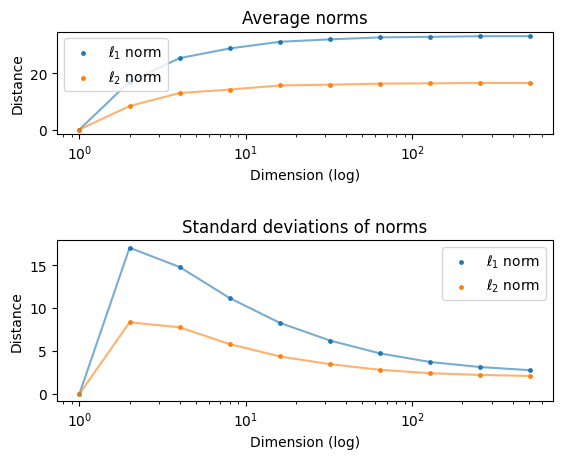
\includegraphics[width=0.6\textwidth]{../q1/figures/output.png}
        \label{fig:q1c}
    \end{figure}

    \item Since expectation is linear:
    
    \[\mathbb{E}(R) = \mathbb{E}(Z_1 + \dots + Z_d) = \sum_{i = 1}^d \mathbb{E}(Z_i) = \frac{d}{6}\]

    Since $Z_i$ are independent and identically distributed, and that variance is additive for independent random variables:

    \[\text{Var}(R) = \text{Var}(Z_1 + \dots + Z_d) = \sum_{i = 1}^d \text{Var}(Z_i) = d \cdot \frac{7}{180}\]

    \item We proceed in steps as justified in the handout. 
    \begin{enumerate}[i. ]
        \item The event ``R is at least $k$ away from its expectation'' can be written as \[E = |R - \mathbb{E}(R)| \geq k\]
        \item Using Markov's inequality, we have that \[\Pr(E) \leq \frac{\text{Var}(R)}{k^2} = \frac{d}{k^2} \cdot \frac{7}{180}\]
        \item If $k = cd$, then we have that \[\Pr(E) \leq \frac{1}{c^2 d} \cdot \frac{7}{180}\]
        With $d \to \infty$, we see that $\Pr(E) \to 0$.
    \end{enumerate}

    This supports the claim that most pairs of points are approximately the same distance. Given fixed $k$ proportional to $d$, we see that the probability of $R$ being at least $k$ away from its expectation goes to 0 as $d$ grows. That is, it is very likely that $R$ is $k$-close to its expectation as $d$ grows. More formally, given fixed $c$, we can find $d$ large enough such that for $k = cd$, we have $P(E) \leq \epsilon$, or $P(|R - \mathbb{E}(R)| < k) >  1 - \epsilon$.
\end{enumerate}

\newpage
\section*{Question 2}

\begin{enumerate}[(a)]
    \item \texttt{load\_data} implemented in the attached file. 
    \item The output of \texttt{select\_model} is attached below, along with a report of the corresponding test accuracy for the best hyperparameters.

    \begin{verbatim}
        Depth  50 with gini     criterion had validation accuracy 0.73673 
        Depth 100 with gini     criterion had validation accuracy 0.75306 
        Depth 150 with gini     criterion had validation accuracy 0.73265 
        Depth 200 with gini     criterion had validation accuracy 0.74286 
        Depth 250 with gini     criterion had validation accuracy 0.74490 
        Depth 300 with gini     criterion had validation accuracy 0.73061 
        Depth  50 with entropy  criterion had validation accuracy 0.73878 
        Depth 100 with entropy  criterion had validation accuracy 0.73061 
        Depth 150 with entropy  criterion had validation accuracy 0.76327 
        Depth 200 with entropy  criterion had validation accuracy 0.75102 
        Depth 250 with entropy  criterion had validation accuracy 0.74694 
        Depth 300 with entropy  criterion had validation accuracy 0.74490 
        Depth  50 with log_loss criterion had validation accuracy 0.74694 
        Depth 100 with log_loss criterion had validation accuracy 0.74490 
        Depth 150 with log_loss criterion had validation accuracy 0.73265 
        Depth 200 with log_loss criterion had validation accuracy 0.74286 
        Depth 250 with log_loss criterion had validation accuracy 0.75510 
        Depth 300 with log_loss criterion had validation accuracy 0.74694 

        A model trained on the best hyperparameters (depth=150, criterion=entropy) had 
        test accuracy 0.773469387755102
    \end{verbatim}

    \item A visualization of the first two layers of the tree with the highest validation accuracy is attached below. 
    
    \begin{figure}[H]
        \centering
        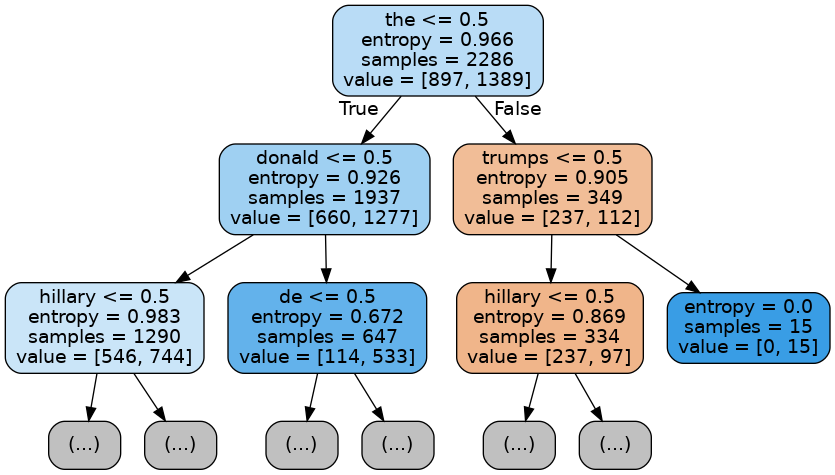
\includegraphics[width=0.6\textwidth]{../q2/figures/best_tree.png}
        \label{fig:q2c}
    \end{figure}

    \item The output of \texttt{compute\_information\_gain} is attached below for the top feature in the figure above, along with three others. 
    
    \begin{verbatim}
        Information gain for feature `the     ` with threshold 0.5 is 0.04388027604368
        Information gain for feature `donald  ` with threshold 0.5 is 0.04286986143652
        Information gain for feature `trumps  ` with threshold 0.5 is 0.04333523607079
        Information gain for feature `hillary ` with threshold 0.5 is 0.03414166828335
    \end{verbatim}

\end{enumerate}


\section*{Question 3}

\newcommand{\J}{\mathcal{\mathcal{J}^{\alpha\beta}_{\text{reg}}}}
\newcommand{\sgn}{\mathcal{\text{sgn}}}

\begin{enumerate}[(a)]
    \item First, if we define 
    
    \[f^\alpha(\mathbf{w}) = \sum_{j' = 1}^D \alpha_{j'} |w_{j'}|\]

    then we have for $w_j \neq 0$ that 

    \begin{align*}
        \frac{\partial f^\alpha}{\partial w_j}(\mathbf{w}) &= \alpha_j \cdot \sgn(w_j)
    \end{align*}

    For the purpose of this question, we will extend the definition of $\sgn$ to be 0 when its argument is 0. In this way, we abuse notation to extend $\partial f^\alpha/\partial w_j(\mathbf{w})$ to be defined as $0$ for $w_j = 0$, even though $f^\alpha$ is not differentiable with respect to $w_j$ at $w_j = 0$.

    Now, we have that

    \begin{align*}
        \J(\mathbf{w}, b) &= \frac{1}{2N} \sum_{i = 1}^N \left(y^{(i)} - t^{(i)}\right)^2 + f^\alpha(\mathbf{w}) + \frac{1}{2} \sum_{j' = 1}^D \beta_j w_{j'}^2\\
        \frac{\partial \J}{\partial w_j}(\mathbf{w}, b) &= \left(\frac{\partial}{\partial w_j}\right) \left(\frac{1}{2N} \sum_{i = 1}^N \left(y^{(i)} - t^{(i)}\right)^2\right) + \left(\frac{\partial}{\partial w_j}\right) f^\alpha(\mathbf{w}) + \left(\frac{\partial}{\partial w_j}\right) \left(\frac{1}{2} \sum_{j' = 1}^D \beta_j w_{j'}^2\right)\\
       &=  \frac{1}{N} \sum_{i = 1}^N x_j^{(i)} \left(y^{(i)} - t^{(i)}\right) + \alpha_j \cdot \sgn(w_j) + \beta_j w_j
    \end{align*}

    and similarly 

    \begin{align*}
        \frac{\partial \J}{\partial b}(\mathbf{w}, b) &= \left(\frac{\partial}{\partial b}\right) \left(\frac{1}{2N} \sum_{i = 1}^N \left(y^{(i)} - t^{(i)}\right)^2\right) + \left(\frac{\partial}{\partial b}\right) f^\alpha(\mathbf{w}) + \left(\frac{\partial}{\partial b}\right) \left(\frac{1}{2} \sum_{j' = 1}^D \beta_j w_{j'}^2\right)\\
         &=  \frac{1}{N} \sum_{i = 1}^N \left(y^{(i)} - t^{(i)}\right) + 0 + 0\\
         &= \frac{1}{N} \sum_{i = 1}^N \left(y^{(i)} - t^{(i)}\right)
    \end{align*}

    and so the gradient descent update rule $w_j \gets w_j - \alpha' \partial \J / \partial w_j$ is given as follows for $j = 1, \dots, D$, with $\alpha'$ the learning rate:

    \begin{itemize}
        \item If $w_j > 0$:
        
        \begin{align*}
            w_j &\gets w_j - \alpha' \left(\frac{1}{N} \sum_{i = 1}^N x_j^{(i)} \left(y^{(i)} - t^{(i)}\right) + \alpha_j + \beta_j w_j\right)\\
            b & \gets b - \alpha' \left(\frac{1}{N} \sum_{i = 1}^N \left(y^{(i)} - t^{(i)}\right)\right)
        \end{align*}

        \item If $w_j = 0$:
    
        \begin{align*}
            w_j &\gets w_j - \alpha' \left(\frac{1}{N} \sum_{i = 1}^N x_j^{(i)} \left(y^{(i)} - t^{(i)}\right) \right)\\
            b & \gets b - \alpha' \left(\frac{1}{N} \sum_{i = 1}^N \left(y^{(i)} - t^{(i)}\right)\right)
        \end{align*}

        \item If $w_j < 0$:
        
        \begin{align*}
            w_j &\gets w_j - \alpha' \left(\frac{1}{N} \sum_{i = 1}^N x_j^{(i)} \left(y^{(i)} - t^{(i)}\right) - \alpha_j + \beta_j w_j\right)\\
            b & \gets b - \alpha' \left(\frac{1}{N} \sum_{i = 1}^N \left(y^{(i)} - t^{(i)}\right)\right)
        \end{align*}
    \end{itemize}
    
    We expect that this form of regularization is called ``weight decay'' because it causes the regularization term to contain a constant term $(\alpha_j)$ that does not grow small even for small non-zero values of $w_j$. This means that unlike just $\ell_2$ regularization, the weights continue to decay significantly even for small non-zero values of $w_j$.

    \item We derive formulae for $A_{j j'}$ and $c_j$ as follows: 
    
    \renewcommand*{\J}{\mathcal{J}^{\beta}_{\text{reg}}}

    \begin{align*}
        \frac{\partial \J}{\partial w_j}(\mathbf{w}) &= \frac{1}{N} \sum_{i = 1}^N x_j^{(i)} \left(y^{(i)} - t^{(i)}\right) + \beta_j w_j\\
        &= \frac{1}{N} \sum_{i = 1}^N x_j^{(i)} \left(\sum_{j' = 1}^D w_{j'} x_{j'}^{i} - t^{(i)}\right) + \beta_j w_j\\
        &= \beta_j w_j + \frac{1}{N} \sum_{i = 1}^N \sum_{j' = 1}^D w_{j'}  x_j^{(i)} x_{j'}^{i}  -  \frac{1}{N}\sum_{i = 1}^N x_j^{(i)} t^{(i)} \\
        &= \beta_j w_j + \sum_{j' = 1}^D \left(\frac{1}{N} \sum_{i = 1}^N x_j^{(i)}x_{j'}^{(i)} \right) w_{j'} -  \frac{1}{N}\sum_{i = 1}^N x_j^{(i)} t^{(i)} \\
        &= \beta_j w_j + \sum_{j' = 1}^D \left(\frac{1}{N} x_j^T x_{j'} \right) w_{j'} -  \frac{1}{N} x_j^T t \\
    \end{align*}

    and so we can write \[A_{jj} = \begin{cases}
        \dfrac{1}{N} x_j^T x_{j'} & j \neq j'\\
        \beta_j + \dfrac{1}{N} x_j^T x_{j'} & j = j'
    \end{cases}
        \]
        \[c_j = \frac{1}{N} x_j^T t\]

    \newcommand{\diag}{\text{diag}}
    \item We can write \[\mathbf{A} = \frac{1}{N} \mathbf{X}^T \mathbf{X} + \diag(\beta)\]
    
    where $\diag(\beta)$ represents the diagonal $D \times D$ matrix which has \[\diag(\beta) = \begin{bmatrix}
        \beta_1 & 0 & \dots & 0\\
        0 & \beta_2 & \dots & 0\\
        \vdots & \vdots & \ddots & \vdots\\
        0 & 0 & \dots & \beta_D
    \end{bmatrix}
        \]
        We see this as follows. The $jj'$ entry of $\frac{1}{N} \mathbf{X}^T \mathbf{X}$ is precisely $x_j^T x_{j'}$. Further, the $jj'$ entry of $\diag(\beta)$ is $\beta_j$ if $j' = j$, and zero otherwise. Thus, their sum gives $A_{jj'}$ as required.

        Further, we can write \[\mathbf{c} = \frac{1}{N} \mathbf{X}^T t\]

        since its $j$th entry is precisely $\frac{1}{N} x_j^T t$.

        Now, we'll derive a closed form solution for $\mathbf{w}$ in terms of $\mathbf{A}$ and $\mathbf{c}$. We would like 

        \[\frac{\partial \J}{\partial w_j} (\mathbf{w}) = \sum_{j' = 1}^D A_{jj'} w_{j'} - c_j = \mathbf{A}_j \mathbf{w} - \mathbf{c}_j = (\mathbf{Aw} - \mathbf{c})_j = 0\]

        for all $j = 1, \dots, D$. This is equivalent to solving the linear system $\mathbf{Aw} = \mathbf{c}$, which has a unique solution if $\mathbf{A}$ is invertible. Indeed, with this assumption, we have \[\mathbf{w} = \mathbf{A}^{-1} \mathbf{c} = \left(\frac{1}{N} \mathbf{X}^T \mathbf{X} + \diag(\beta)\right)^{-1}\left(\frac{1}{N} \mathbf{X}^T t\right) = \left(\mathbf{X}^T \mathbf{X} + N \diag(\beta)\right)^{-1}\left(\mathbf{X}^T t\right)\] 
\end{enumerate}

\end{document}